\subsubsection{遅延とパケット損}

各ノード(ルータ)における遅延

\begin{itemize}
  \item 処理遅延: パケットのヘッダを読み、出力リンクを決定する時間\\
    伝送誤りチェックも含む\\
    (通常 $ns \sim \mu s$ のオーダ)\\
    \textcolor{cyan}{パリティチェック等}
  \item 待ち行列遅延: 送信待ちに要する時間\\
    (通常 $100ms$ 程度まで、バッファサイズに依存)\\
    \textcolor{cyan}{LAN出力ポートに複数の出力が来た際の待ち時間、バッファサイズによってパケットを保持できる(より情報を保持できるが待ち時間も増える)}
  \item 伝送遅延: パケットを通信リンクに送り出す時間\\
    (リンクの容量を $R[\rm{bps}]$, パケットサイズを $L\; \rm{bit}$ とすると, $\displaystyle \frac{L}{R}$)
  \item 伝搬遅延: 送信された 1 ビット目の情報が次のノードに到達するまでの時間\\
    (光速より少し遅め、 $2 \times 10^8 m/s \sim 3 \times 10^8 m/s$ 程度)\\
    \textcolor{cyan}{ex.) 衛星通信など。送信元と送信先の距離によって変化}
\end{itemize}
\underline{パケット損}

待ち行列(バッファ)に入ることのできるパケットの数は有限
\begin{itemize}
  \item[$\Rightarrow$] パケット損が生じる
\end{itemize}
一般に、「バッファサイズ大」 $\Leftrightarrow $ 「待ち行列遅延大 かつ パケット損小」\\
というトレードオフが存在

\textcolor{cyan}{パケットの損失はTCPの場合、輻輳制御によってサービスが低下する}


\subsubsection{ルーチング}

送信ホストは終点ホストのアドレス(IPアドレス)をパケットのヘッダに書き込んで送信

ルータは、終点アドレスを出力リンクに対応付けた \textcolor{orange}{ルーチングテーブル} を持ち、検索して転送

\indent\indent\textcolor{cyan}{ネットワークグラフの情報を持っていて、適切な経路を返すイメージ?}

ルータはコネクション情報を管理しない(ヘッダに書かれたアドレスを読むだけ)

ルーチングテーブルの自動作成
\begin{itemize}
  \item[$\Rightarrow$] \textcolor{orange}{ルーチングプロトコル}
\end{itemize}
% フォアディング、アドレッシング

\newpage
\subsubsection{ネットワークのネットワーク}
インターネット (the Internet) は、複数の ISP 同士が階層的に接続することで構成

\indent\textcolor{orange}{ネットワークのネットワーク (Network of network)}

\textcolor{cyan}{イントラネット(企業内などの閉じたインターネット)、ARPANETから始まったインターネットが大きな塊になっていった}

\begin{itemize}
  \item アクセスISP: DSL, FTTH, Wi-Fi, セルラ, ビジネスLANなどによるエンドシステムからのアクセスを提供\\
    \textcolor{cyan}{DSL: 日本では ADSL(asymmetric DSL)}
  \item Tier1 ISP: 他の Tier1 ISPおよび下位ISPと接続し、国際的エリアをカバー\\
    \textcolor{cyan}{日本ではNTTコミュニケーションズとソフトバンクの2社}
  \item Tier2 ISP(広域), Tier3 ISP(地域):
  \begin{itemize}
    \item[] Tier2 ISPは、グローバル通信を行うとき、Tier1 ISPを介してトランジット通信
    \item[] 上位ISPはサービスプロバイダ、下位ISPはカスタマーという関係となり、トラヒック量に応じて料金を課す(従量課金)
  \end{itemize}
  \textcolor{cyan}{ISP: Internet survice provider, 通信の企業のことみたい。kddi $\rightarrow$ so-net $\rightarrow$ user みたいな感じ?}
\end{itemize}

\begin{itemize}
  \item ピアリング:
  \begin{itemize}
    \item[] 同層ISP間で接続すること。
    \item[] 上位ISPへのトランジット料金の支払いを軽減
  \end{itemize}
  \item  相互接続点(PoP: Point of Presence): ISP間が接続するときの接続点\;(複数のルータから構成)\\
  \textcolor{cyan}{複数の事業者間で通信するには物理的にルータが繋がっている必要がある}
  \item IXP(Internet Exchange Point): ピアリングするISPがつなぎこむ箇所を提供する、独立した組織\\
  \textcolor{cyan}{PoPを提供する事業者}
  \item コンテンツプロバイダ:
  \begin{itemize}
    \item Googleなど、非常に大きなリソースを持つサードパーティ (\textcolor{orange}{Hypergiants}などとも呼ばれる)
    \item Tier2, Tier3 ISP と直接ピアリングを行う
    \item[] \textcolor{cyan}{従量課金がなくなるため、下位ISPとしてもWin-Win}
  \end{itemize}
\end{itemize}

\begin{figure}[h]
  \centering
  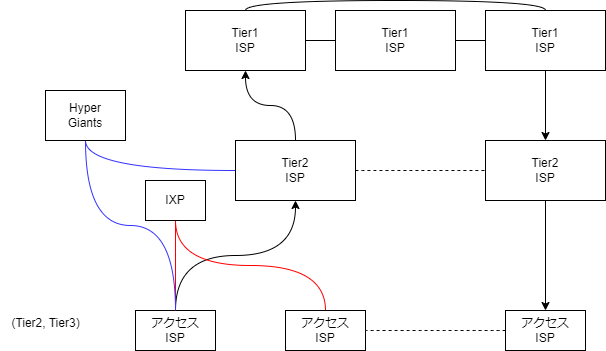
\includegraphics[width=0.6\linewidth]{image/isp.png}
  % \caption{}
  % \label{fig:}
\end{figure}
